\subsection{Voting for Participant Identification}
\label{vote}
\vspace{-5pt}
The next step is to accumulate participant information from noisy instantaneous matches $W^{t,s}$, with the goal of identify a single optimized matching matrix, denoted $W^{*}\in\mathcal{W}$, that identifies a single consistent set of $N<M$ participants over the duration of the interaction. We achieve this through voting, with the intuition being that the optimal matching $W^{*}$ will occur relatively frequently among the instantaneous matches $\{W^{t,s}\}$. 

The scenario now resembles the setting for a general Hough Transform, where the desired parameters are supported by the maximum number of image feature observations: A parameter set and an observation set are established, for every observation one enumerates over all parameters and determines every parameter that is compatible with the observation, the count for that compatible parameter in an accumulator array for all parameters is increased by one, and finally the parameter receiving the maximum number of counts is reported. Here, we regard the parameter set as consisted of two parts - the set of all possible matchings $\mathcal{W}$ and the exemplar $\mathcal{D}$, and we regard the observation set as the input $\mathcal{Q}$. However, note that the overall optimal matching may not simply be achieved on the matching receiving the maximum number of counts, but on the matching which yields the maximum similarity with the exemplar. Therefore, in addition to maintaining an accumulator array for the counts on all matchings $\mathcal{W}$, we also maintain a companion accumulator array for the corresponding dissimilarity measures achieved by these matchings. 

\begin{figure}[t]
\vspace{-5pt}
\begin{center}
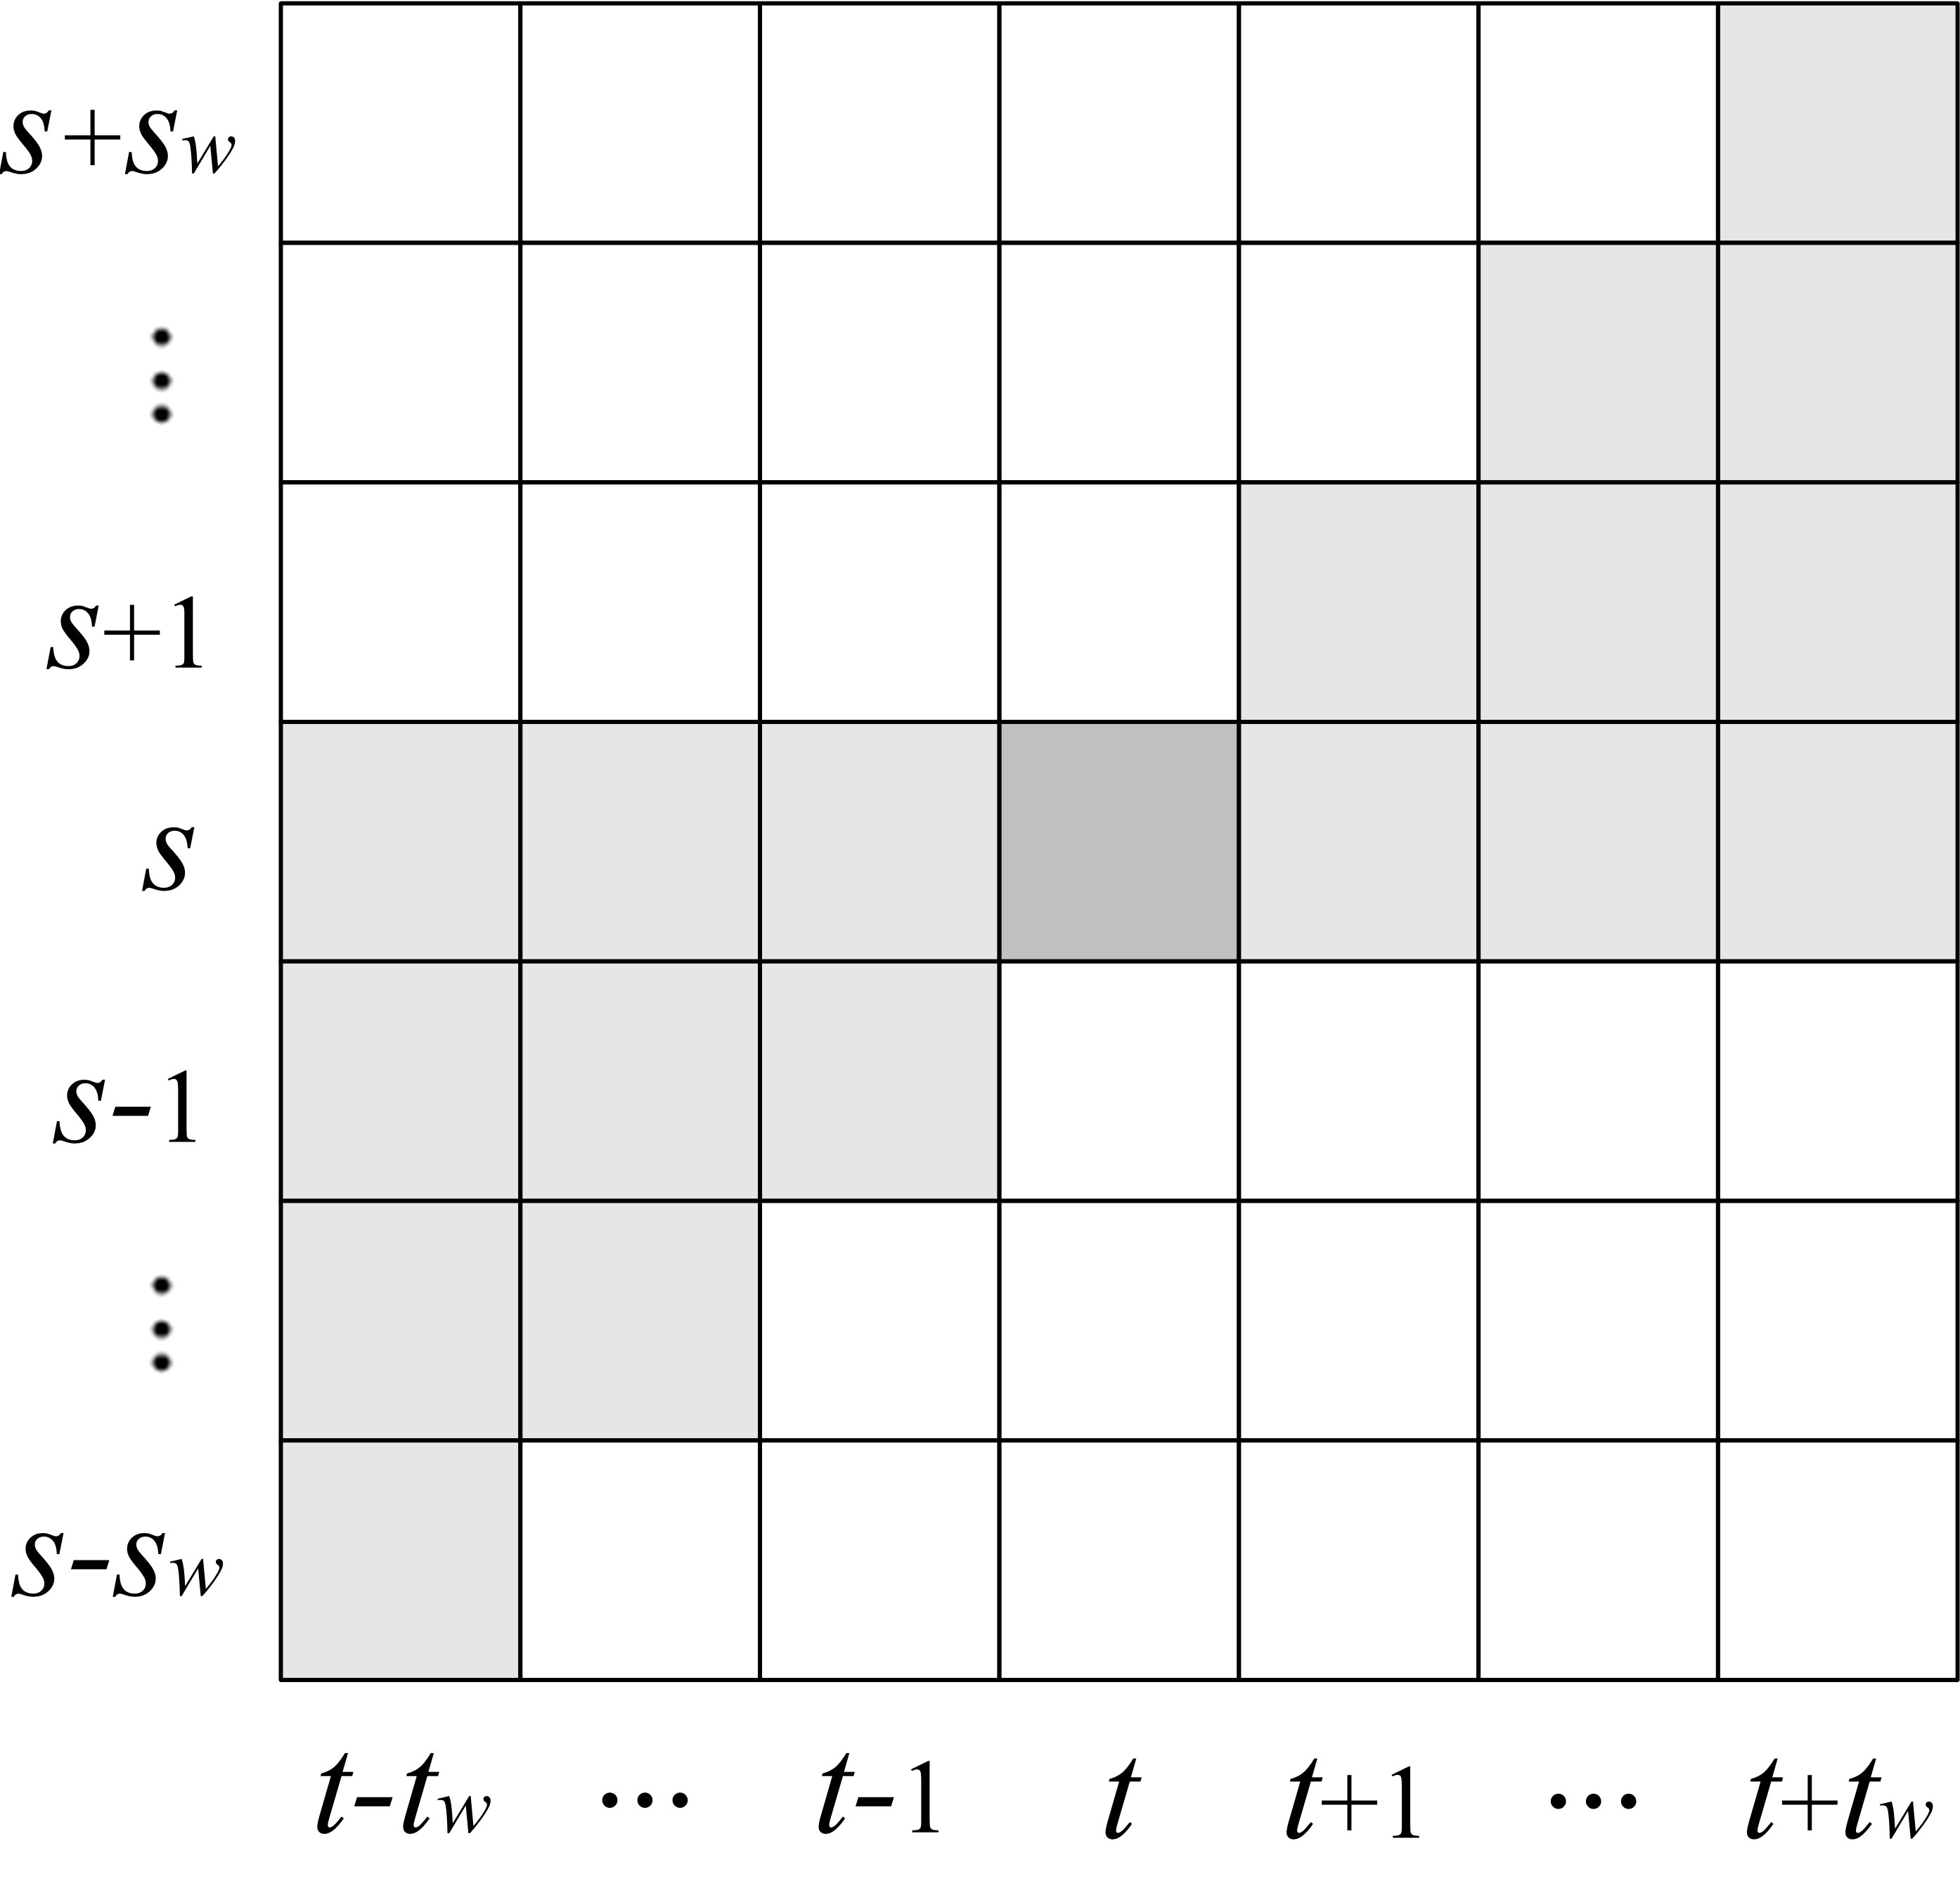
\includegraphics[scale=0.3]{neighbor2.png}
\end{center}
\caption{The temporal neighborhood used in to compute (\ref{softvote}). See Sec. \ref{vote} for details.}
\label{all_illu}
\vspace{-5pt}
\end{figure}

Given the above considerations, two efforts are made in order to allow $W^{*}$ to emerge from the instantaneous matchings $W^{t,s}$'s. First, through metric learning to be presented in Sec. \ref{MetLearn}, we pursue the effect that the dissimilarity $D(\mathcal{Q}_{t}, \mathcal{D}_{s})$ yields a smaller number if the optimal $N$ agents in $\mathcal{Q}_{t}$ better matches with $\mathcal{D}_{s}$, and yields a larger number otherwise. Second, instead of directly using the dissimilarity scores $D(\mathcal{Q}_{t}, \mathcal{D}_{s})$ for the companion accumulator array, we consider the fact that if the matching $W^{t,s}$ is optimal at time pair $(t,s)$, the optimal matchings at the temporally nearby (input, exemplar) time pairs should be also achieved by the same matrix $W^{t,s}$. This means that the matching matrices of these nearby times should all agree, and their dissimilarities $D$'s should all be small. Therefore, we use the follow temporal-consistency preserved dissimilarity measure to vote in the companion array for $W^{t,s}$
\begin{equation}
\vspace{-5pt}
\label{softvote}
v(W^{t,s})=\sum_{(t',s')\in\mathcal{N}(t,s)}(\|W^{t,s}-W^{t',s'}\|_{1}+1)D(\mathcal{Q}_{t'}, \mathcal{D}_{s'}).
\end{equation}
Here $\mathcal{N}(t,s)$ is a temporal neighborhood of $(t,s)$ in which we enforce the consistency and it is depicted in Fig. \ref{all_illu} (a), where the pair $(t,s)$ is shown in black square and the neighborhood is shown in shaded area. Neighborhood sizes $t_{w}$ and $s_{w}$ are taken as a quarter of the length of a cell on the bottom of the pyramid (See Sec. \ref{BB})\footnote{When the neighborhood extends out of video boundary, we only consider the cells within the boundary and normalize the vote by the number of cells actually involved.}. (\ref{softvote}) implies that, when evaluating the vote $v(W^{t,s})$ for input time $t$ against exemplar time $s$, we also look at the interactive behavior happening ahead of (resp. after) $t$, and expect that the two aforementioned consistencies are maintained so that the the interactive behaviors happening ahead of (resp. after) $t$ resembles that happening ahead of (resp. after) $s$ in the exemplar, in the sense of a smaller $D$ and a same matching matrix. Eventually, a better matching will receive a lower vote $v$.
\vspace{-10pt}
\begin{algorithm}
\footnotesize{
\begin{enumerate}
\item Clear both accumulator arrays;
\item For each $t\in[1,T], s\in[1,S]$, increment the count for the matching matrix $W^{t,s}$ by 1, and increase the vote in the\\ 
companion array corresponding to $W^{t,s}$ by $v(W^{t,s})$;
\item Identify a subarray of matrices receiving more than $\frac{S}{2}$ counts, \\
and normalize the dissimilarity votes in the companion subarray 
\\by corresponding counts;
\item Report the matching matrix $W^{*}$ to be the one in the subarray receiving the minimum normalized dissimilarity vote.
\end{enumerate}
}
\caption{\small Voting procedure for identify the participants (\textit{i.e.}, the best overall matching $W^{*}$).}
\label{Algo:1}
\end{algorithm}
\vspace{-10pt}

 As a result, the voting procedure is shown in Algorithm \ref{Algo:1}, where in the last two steps we find among those matching matrices which receive a substantial number of supports from instantaneous matchings the best matching $W^{*}$ with the lowest average dissimilarity to the exemplar. This idea is also illustrated in Fig. \ref{diagram}, where a thick matching line indicates a strong similarity (low vote $v$), and the agents receiving the average lowest votes are selected as participants.


